\newpage
\begin{textblock*}{3cm}(0cm,-1cm) % {block width} (coords)
    \begin{tikzpicture}
        \fill[ERDCRed] (0,0) rectangle (3,29.1); % Fill for the sidebar
        \draw[white, thick] (0.1,0.1) rectangle (2.9,29.11); % White border for aesthetic
    \end{tikzpicture}
\end{textblock*}

% Add vertical text for the book title
\begin{textblock*}{40cm}(1cm,10cm) % Adjust the width and position of the text block to accommodate larger text
    \rotatebox{90}{
        \fontsize{40}{48}\selectfont % Adjusted for better fit
        \textbf{\color{white}Part One} % Change text here
    }
\end{textblock*}

\newgeometry{left=5.81cm, top=1in, bmargin=1in, right=1in}
\begin{center}
\section{Design \hspace{0.5cm} \color{white}1} 
\end{center}
This system attempts to create a more noise-conscious environment in libraries by communicating to users their noise level in various ways. The display presents a top-down view of the library, with desks coloured according to the live noise level output. Users have the ability to send anonymous text-like messages to other desks to politely ask them to be quieter. There is also a volume metre and decibel count to indicate the noise level to users. By also using quiet auditory cues and gentle vibrations through the desk, disruptive individuals can be made aware of their noise output without disturbing others. This multimodal approach uses as many methods as possible to grab attention and also accommodates a variety of users, including those with sensory impairments.
\begin{figure}[h]
    \centering
\frame{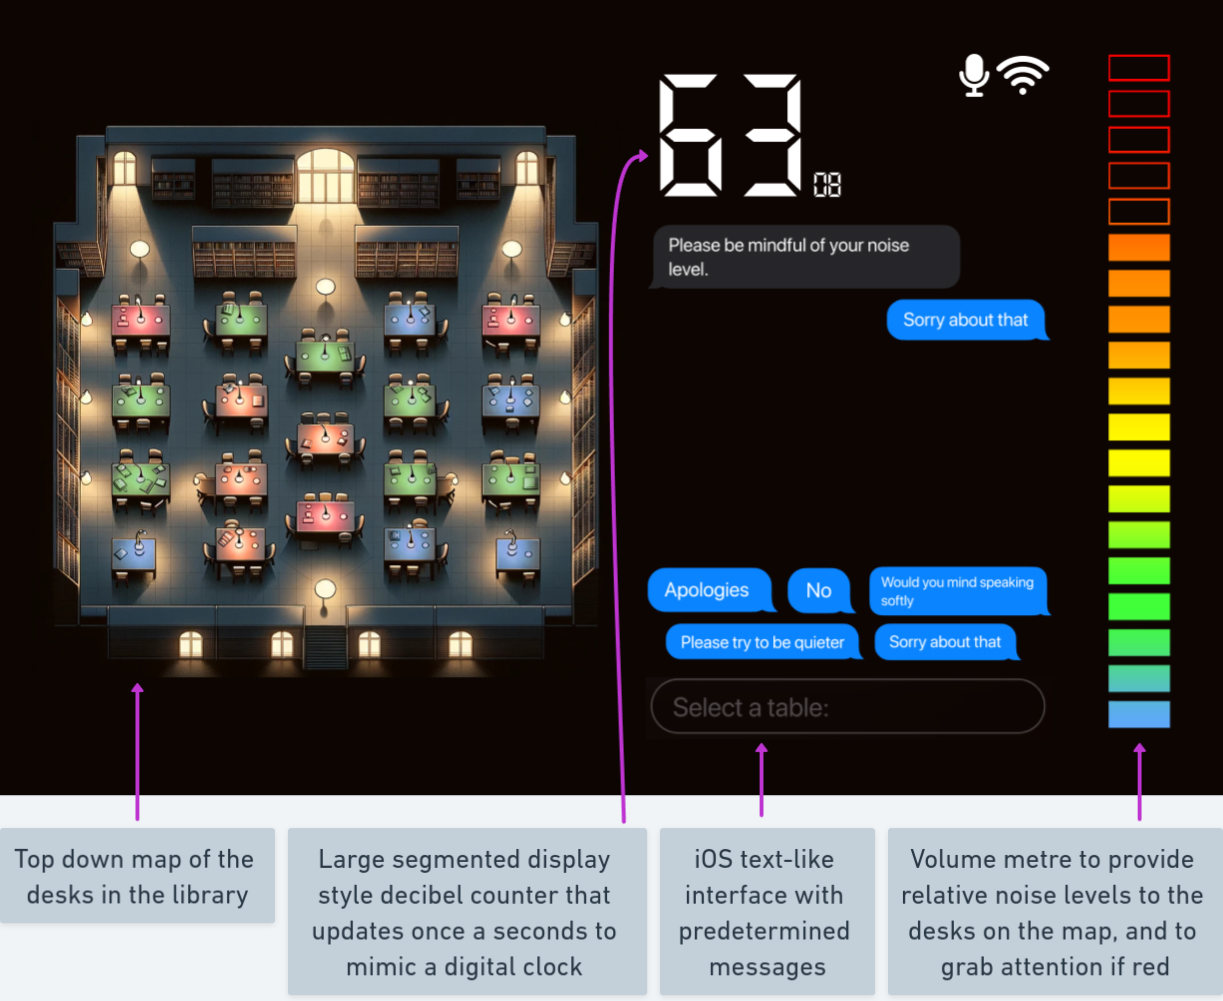
\includegraphics[width=\textwidth]{images/design}}
\caption{Display of the System}
\end{figure}
\restoregeometry

